\PassOptionsToPackage{quiet}{fontspec}
\documentclass[12pt,a4paper,UTF8]{article}
\usepackage{thesis} % 格式控制
\setlength{\parindent}{2em} % 控制首行缩进  
\addtolength{\parskip}{3pt} % 控制段落距离  
\onehalfspacing % 1.5倍行距  
\graphicspath{{./figures/}} % 指定图片所在文件夹  
\usepackage{dirtree}

\usepackage{xeCJK} % 支持中文
\classname{智能控制技术}  % 设置课程名称
\expname{HW03 模糊控制}
\makepagestyle{\printexpname}{\printclassname ~实验报告}

\begin{document}
\maketitlepage{\printexpname}{教7 304}{PhilFan}{19260817}{\today}{刘山} %封面页 

\maketoc    %目录页
\section{实验目的和要求}
\subsection{实验目标}
\begin{enumerate}
\item 系统方程:
\begin{equation}
F - G = m \frac{d^2 X}{dt^2}
\end{equation}

其中,$F$ 为电磁吸力,$m$ 为钢球的质量,重力 $G = mg$,$g$ 为重力加速度。

\item 电磁力方程:
\begin{equation}
F = K \left( \frac{I}{X} \right)^2
\end{equation}

其中,$K$ 为电磁力系数。

\item 电磁线圈方程:
\begin{equation}
U - K \frac{I}{X} \frac{dX}{dt} = L \frac{dI}{dt} + IR
\end{equation}

其中,$U$ 为控制电压,$L$ 为电感,$R$ 为线圈电阻。
\end{enumerate}

假定系统参数如下表所示:

\begin{table}[htbp]
\centering
\begin{tabular}{|c|c|}
\hline
参数 & 值 \\
\hline
$m$ & 0.05kg \\
$g$ & 9.81m/$s^2$ \\
$K$ & 0.005 $N m^2/A^2$ \\
$R$ & 5$\Omega$ \\
$L$ & 0.01$H$ \\
\hline
\end{tabular}
\end{table}

请完成以下任务:
\begin{problem}
\begin{enumerate}
\item \textbf{推导磁悬浮系统的状态空间模型:}(提示:以钢球位置 $X$、速度 $\dot{X}$ 和电流 $I$ 为状态变量)

\item \textbf{针对上述磁悬浮系统,设计模糊控制器使钢球位置稳定在期望位置 $X_d = 0.05m$。} 假设初始钢球位置为 $X(0) = 0.03m$,初始速度和初始电流均为 0,仿真实现系统的模糊控制,绘制钢球位置随时间变化曲线、控制电压随时间变化曲线,并分析仿真结果。(输入输出的论域范围自行选择,可尝试位置误差范围 [-0.04,0.04]m,位置误差变化率范围 [-0.5,0.5]m/s,控制电压的范围 [-10,10]V)

\item \textbf{若改变钢球质量为 0.1kg,其他参数不变,重新进行仿真并分析对系统控制性能的影响,讨论如何调整模糊控制器参数以适应钢球质量的变化。}
\end{enumerate}
\end{problem}

\section{问题建模分析}
\begin{enumerate}
\item \textbf{系统的非线性特征}\\
磁悬浮系统作为一个典型的非线性复杂系统,磁悬浮系统可以通过两种方式进行控制:一是在特定工作点进行局部线性化后应用线性控制方法,二是直接采用非线性控制理论进行系统设计。

\item \textbf{系统的不确定性}\\
磁悬浮系统运行过程中存在模型误差、电磁干扰以及其他外部环境因素的影响。

\item \textbf{系统的开环不稳定性}\\
系统仅在电磁力与重力达到平衡时存在唯一的稳定状态,且这种平衡必须在闭环控制下才能维持。在开环状态下,即使极小的外部扰动也会导致系统失去平衡
\end{enumerate}
    

\subsection{状态方程}
根据系统的动力学方程,我们可以推导状态空间模型。选取状态变量:
\begin{equation}
\begin{aligned}
x_1 &= X \\
x_2 &= \dot{X} = \frac{dX}{dt} \\
x_3 &= I
\end{aligned}
\end{equation}

从机械运动方程可得:
\begin{equation}
m\frac{d^2X}{dt^2} = K\left(\frac{I}{X}\right)^2 - mg
\end{equation}

整理得到状态方程:
\begin{equation}
\begin{aligned}
\dot{x}_1 &= x_2 \\
\dot{x}_2 &= \frac{K}{m}\left(\frac{x_3}{x_1}\right)^2 - g \\
\dot{x}_3 &= \frac{1}{L}\left(U - K\frac{x_3}{x_1}x_2 - Rx_3\right)
\end{aligned}
\end{equation}

其中,$x_1$为钢球位置,$x_2$为钢球速度,$x_3$为电流。这是一个非线性系统的状态空间表达式。

\newpage
\subsection{物理系统的S-function实现}

根据系统的动力学方程,和上述的状态方程,可以写出物理系统的S-function表达。

\begin{lstlisting}[language=Matlab,caption=物理系统的S-function实现]
function [sys, x0, str, ts, simStateCompliance] = mdlInitializeSizes()
    % 初始化回调子函数
    
    sizes = simsizes;
    sizes.NumContStates = 3;   % 连续状态数
    sizes.NumDiscStates = 0;   % 离散状态数:[theta_min, cost_function]
    sizes.NumOutputs = 2;      % 输出个数
    sizes.NumInputs = 1;       % 输入个数
    sizes.DirFeedthrough = 0;  % 允许直馈通道
    sizes.NumSampleTimes = 1;  % 采样时间数
    sys = simsizes(sizes);     % 返回sizes数据结构
    x0 = [0.03 0 0];             % 初始状态:
    str = [];                  % 保留参数
    ts = [0 0];                % 采样时间
    simStateCompliance = 'UnknownSimState'; % 仿真状态合规性
end

function sys = mdlDerivatives(t, x, u,m,g,K,R,L)
    % 导数回调子函数(不使用,空实现)
    xx = x(1);
    dx = x(2);
    I = x(3);
    

    x_dot = dx;
    x_dot2 = (K * I^2 / xx^2 - m*g)/m;
    I_dot = (u - K*I/xx*dx - I*R)/L;
    
    %disp(u)
    %disp([x_dot;x_dot2;I_dot]);
    %disp(xx);
    sys = [x_dot;x_dot2;I_dot];
end
\end{lstlisting}

这里由于是实现物理系统,所以s-funtion可以直接使用非线性的公式,无需进行线性化处理。


\begin{figure}[htbp] \centering 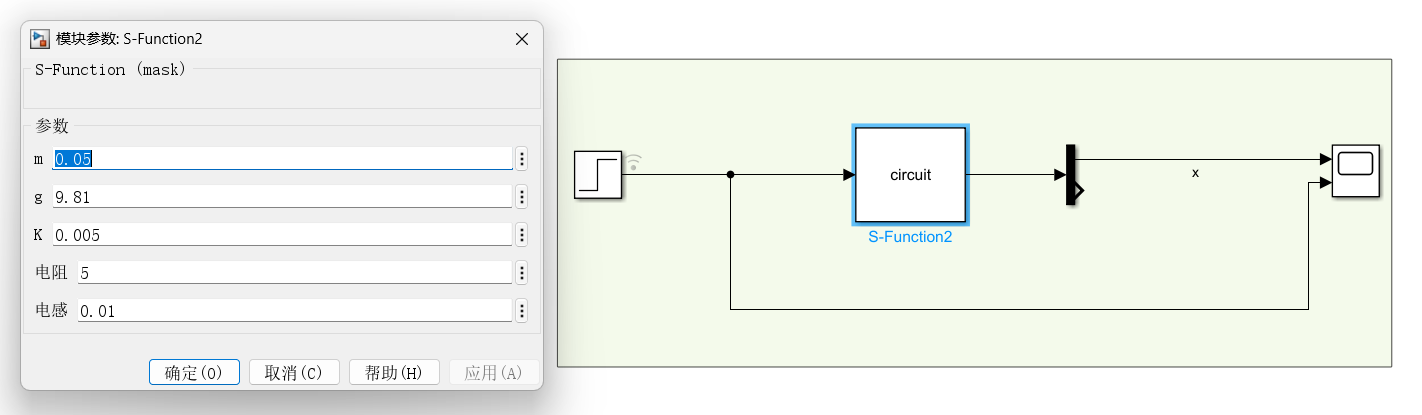
\includegraphics[width=0.9\textwidth]{figures/2024-12-13-21-34-23.png} \caption{搭建的物理模型图}  \end{figure}

搭建好物理模型后,我使用之前学习的Mask的方法,为模型添加了可以直接在simulink中修改参数的界面,无需进入代码即可修改参数


\clearpage % 换页
\section{算法设计}



\textbf{模糊控制的基本概念}

\textbf{模糊控制的定义}
\begin{itemize}
    \item 是将模糊数学理论应用于自动控制领域的控制方法
    \item 基于模糊集合理论、模糊语言变量及模糊逻辑推理
\end{itemize}

\textbf{工作原理}
\begin{itemize}
    \item 通过观察过程输出精确量转化为模糊量
    \item 经过人脑思维与逻辑推理进行模糊判决
    \item 将判决结果的模糊量转化为精确量
\end{itemize}

\textbf{控制特性}
\begin{itemize}
    \item 属于非线性控制
    \item 不依赖于控制对象的精确模型
    \item 仅依靠少量控制规则
    \item 具有较强的鲁棒性
    \item 适用于数学模型未知、复杂的非线性系统控制
\end{itemize}

根据系统逻辑,将系统slx模型搭建如下

\begin{figure}[htbp] \centering 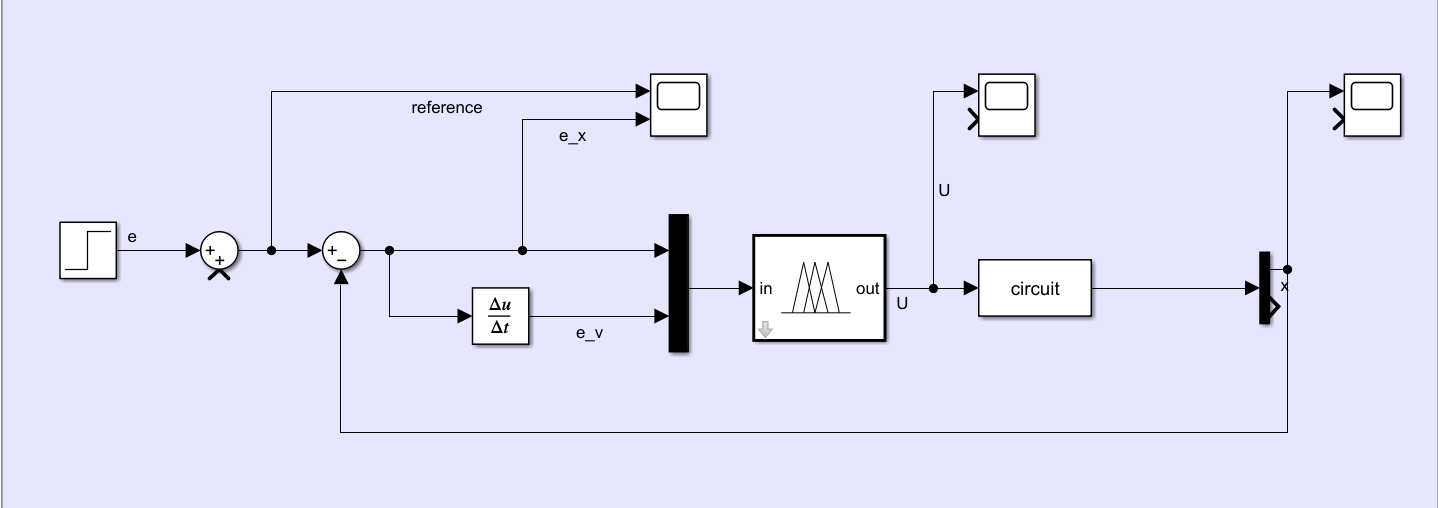
\includegraphics[width=0.9\textwidth]{figures/2024-12-13-21-31-56.png} \caption{系统模型图}\end{figure}
快
\subsection{模糊规则的建立与选择 fuzzy rules}

在刚建立的时候,我感觉上课讲的步骤都是在ui界面下进行操作的,所以就上网搜索了一下如何使用代码建立。

$x$,$v$和$U$我都设置的是高斯函数

\begin{lstlisting}
clear;
close all;

% 创建模糊推理系统,使用 newfis
fuzzyController = mamfis( ...
    'NumInputs',1,'NumInputMFs',2,...
    'NumOutputs',1,'NumOutputMFS',2,...
    'AddRule','none');

% 定义输入变量x(位置误差)及其隶属度函数,范围 [-0.04, 0.04]
fuzzyController.Inputs(1).Name = 'x';
fuzzyController.Inputs(1).Range = [-0.04 0.04];

fuzzyController = addMF(fuzzyController, 'input', 1, 'EN', 'gaussmf', [0.01 -0.04]); % EN: Extremely Negative
fuzzyController = addMF(fuzzyController, 'input', 1, 'VN', 'gaussmf', [0.01 -0.03]); % VN: Very Negative
fuzzyController = addMF(fuzzyController, 'input', 1, 'N', 'gaussmf', [0.01 -0.02]);  % N: Negative
fuzzyController = addMF(fuzzyController, 'input', 1, 'NZ', 'gaussmf', [0.01 -0.01]); % Z: Zero
fuzzyController = addMF(fuzzyController, 'input', 1, 'PZ', 'gaussmf', [0.01 0.01]);  % Z: Zero
fuzzyController = addMF(fuzzyController, 'input', 1, 'P', 'gaussmf', [0.01 0.02]);   % P: Positive
fuzzyController = addMF(fuzzyController, 'input', 1, 'VP', 'gaussmf', [0.01 0.03]);  % VP: Very Positive
fuzzyController = addMF(fuzzyController, 'input', 1, 'EP', 'gaussmf', [0.01 0.04]);  % EP: Extremely Positive

% 可视化x的隶属度函数
figure;
subplot(311);
plotmf(fuzzyController, 'input', 1);
title('位置误差 (x) 的隶属度函数');

% 定义输入变量dx/dt(位置误差变化率)及其隶属度函数,范围 [-0.5, 0.5]
fuzzyController.Inputs(2).Name = 'dx';
fuzzyController.Inputs(2).Range = [-0.5 0.5];
fuzzyController = addMF(fuzzyController, 'input', 2, 'EN', 'gaussmf', [0.1 -0.5]);  % EN: Extremely Negative
fuzzyController = addMF(fuzzyController, 'input', 2, 'VN', 'gaussmf', [0.1 -0.4]);  % VN: Very Negative
fuzzyController = addMF(fuzzyController, 'input', 2, 'N', 'gaussmf', [0.1 -0.3]);  % N: Negative
fuzzyController = addMF(fuzzyController, 'input', 2, 'NZ', 'gaussmf', [0.1 -0.1]);     % Z: Zero
fuzzyController = addMF(fuzzyController, 'input', 2, 'PZ', 'gaussmf', [0.1 0.1]);     % Z: Zero
fuzzyController = addMF(fuzzyController, 'input', 2, 'P', 'gaussmf', [0.1 0.3]);   % P: Positive
fuzzyController = addMF(fuzzyController, 'input', 2, 'VP', 'gaussmf', [0.1 0.4]);   % VP: Very Positive
fuzzyController = addMF(fuzzyController, 'input', 2, 'EP', 'gaussmf', [0.1 0.5]);   % EP: Extremely Positive

% 可视化dx/dt的隶属度函数

subplot(312);
plotmf(fuzzyController, 'input', 2);
title('位置误差变化率 (dx/dt) 的隶属度函数');

% 定义输出变量U(控制电压)的隶属度函数,范围 [-10, 10]
fuzzyController = addvar(fuzzyController, 'output', 'U', [-10 10]);
fuzzyController = addMF(fuzzyController, 'output', 1, 'EL', 'trimf', [-10 -10 -7]);  % EL: Extremely Low
fuzzyController = addMF(fuzzyController, 'output', 1, 'VL', 'trimf', [-10 -7 -4]);  % VL: Very Low
fuzzyController = addMF(fuzzyController, 'output', 1, 'L', 'trimf', [-7 -4 -1]);   % L: Low
fuzzyController = addMF(fuzzyController, 'output', 1, 'NZ', 'trimf', [-3 -1 1]);  % NZ:negetive ZERO
fuzzyController = addMF(fuzzyController, 'output', 1, 'PZ', 'trimf', [-1 1 3]);  % M: positive ZERO
fuzzyController = addMF(fuzzyController, 'output', 1, 'H', 'trimf', [1 4 7]);  % H: High
fuzzyController = addMF(fuzzyController, 'output', 1, 'VH', 'trimf', [4 7 10]); % VH: Very High
fuzzyController = addMF(fuzzyController, 'output', 1, 'EH', 'trimf', [7 10 10]); % EH: Extremely High
\end{lstlisting}

但是值得注意的是,根据调试信息可以看出,这种方法已经逐步被淘汰了,在接下来的版本当中将全被替换成为ui界面操作

\subsection{模糊规则矩阵}
其实使用代码生成模糊矩阵比手动一个个点还是要快一些的,这也是我为什么选择这种方法的原因。


这里我使用了另一个课本中给出的一个参考8x8矩阵作为调参的backbone,在下一节中,我将在这个的基础上进行调参和修改。


\begin{lstlisting}[language=Matlab,caption=生成规则矩阵]
fuzzyController = readfis('Controller4.fis');

table = [
    [1, 1, 1, 1, 6, 5, 5, 5],
    [1, 2, 2, 1, 7, 5, 5, 5],
    [2, 2, 2, 1, 2, 6 ,6, 6],
    [2, 3, 3, 2, 7, 6, 6, 6],
    [3, 3, 3, 2, 8, 7, 6, 7],
    [3, 3, 4, 2,8, 7, 7, 7],
    [3, 4, 4, 2, 8, 8, 7, 8],
    [4, 4, 4, 4, 8, 8, 8, 8]];
% 生成规则矩阵
rules = [];
for i = 1:8
    for j = 1:8
        disp(table(i,j));
        output = table(i,j);
        rules = [rules; i j  output 1 1]; % 1 1表示使用 'min' 合成和 'centroid' 解模糊
    end
end

% disp(rules)

% 添加规则到模糊系统
fuzzyController = addrule(fuzzyController, rules);
%showrule(fuzzyController,'Format','symbolic');
\end{lstlisting}



\begin{lstlisting}[language=Matlab,caption=可视化规则]
% 可视化规则
ruleview(fuzzyController);

%figure;
%plotfis(fuzzyController);

% 输出 surface
figure;
gensurf(fuzzyController,[1,2],1);
saveas(gcf, 'surf.jpg');

% 保存为.fis文件
writefis(fuzzyController, 'Controller41.fis');
\end{lstlisting}

\begin{figure}[htbp] \centering 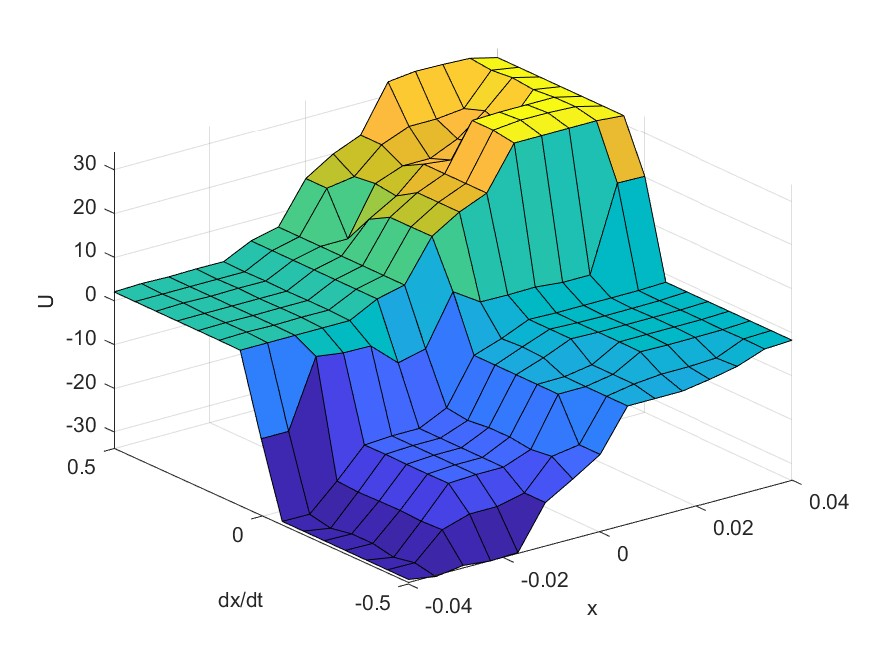
\includegraphics[width=0.7\textwidth]{figures/2024-12-13-22-06-11.png} \caption{模糊控制平面}  \end{figure}

我们可以将surf打印出来。

\newpage
\subsection{模糊规则的调整}

建立了初步的规则,我就在系统上进行了尝试,但是发现效果并不好,经常会出现不收敛、不稳定、震荡大等问题。

所以需要对规则进行调整。


经过反复多次的修改和尝试,最后得到了一版规则

\begin{figure}[htbp] \centering 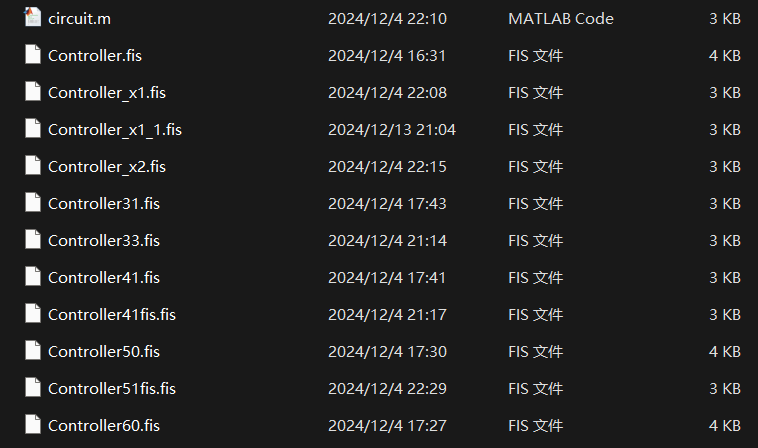
\includegraphics[width=0.7\textwidth]{figures/2024-12-13-22-12-39.png} \caption{经过了反复修改和迭代模型}  \end{figure}


\begin{figure}[!htbp]
    \centering
    \subcaptionbox{surface图片}[0.33\textwidth][c]{
        \centering
        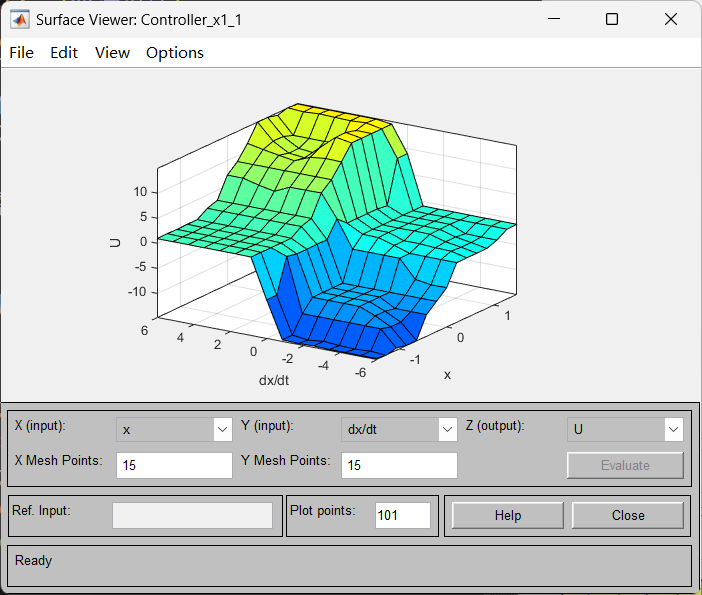
\includegraphics[width=0.32\textwidth]{figures/2024-12-13-22-13-43.png} 
         
    }%
        \subcaptionbox{rules图片}[0.33\textwidth][c]{
        \centering
        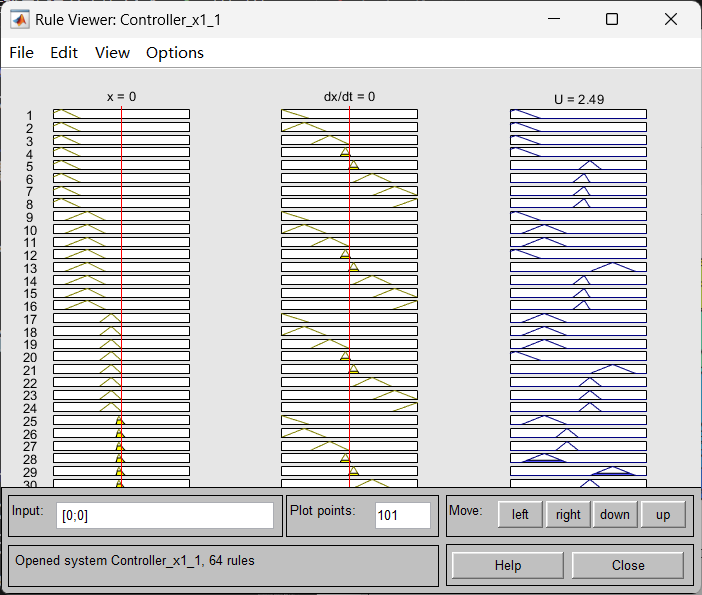
\includegraphics[width=0.32\textwidth]{figures/2024-12-13-22-14-17.png} 
         
    }%
        \subcaptionbox{fis文件}[0.33\textwidth][c]{
        \centering
        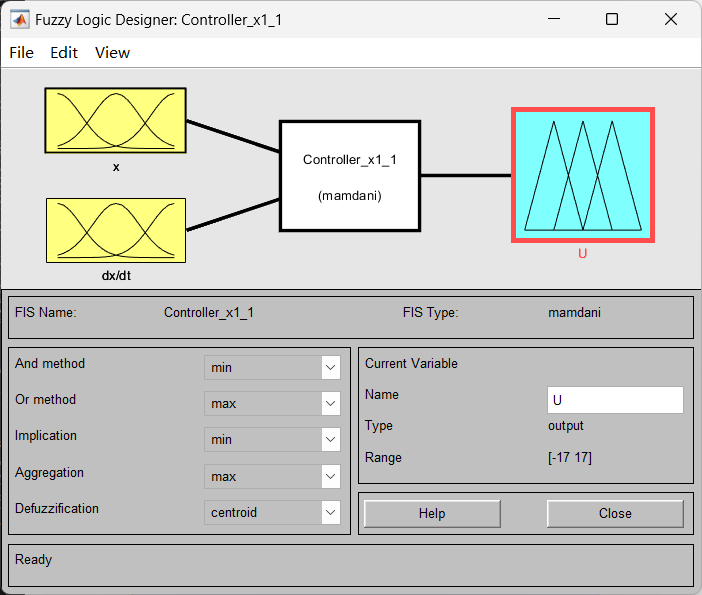
\includegraphics[width=0.32\textwidth]{figures/2024-12-13-22-14-35.png} 
         
    }%
    \caption{最终fis文件}
     
\end{figure}

\begin{figure}[!htbp]
    \centering
    \subcaptionbox{x}[0.33\textwidth][c]{
        \centering
        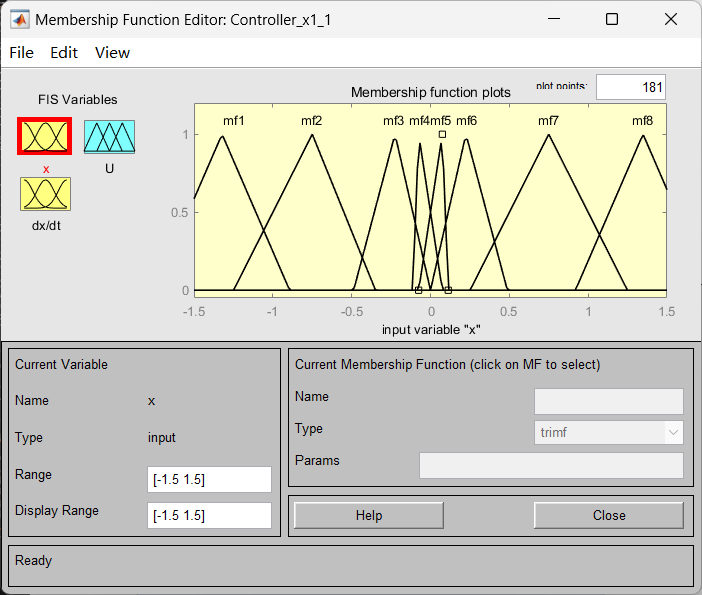
\includegraphics[width=0.32\textwidth]{figures/2024-12-13-22-15-10.png} 
         
    }%
        \subcaptionbox{v}[0.33\textwidth][c]{
        \centering
        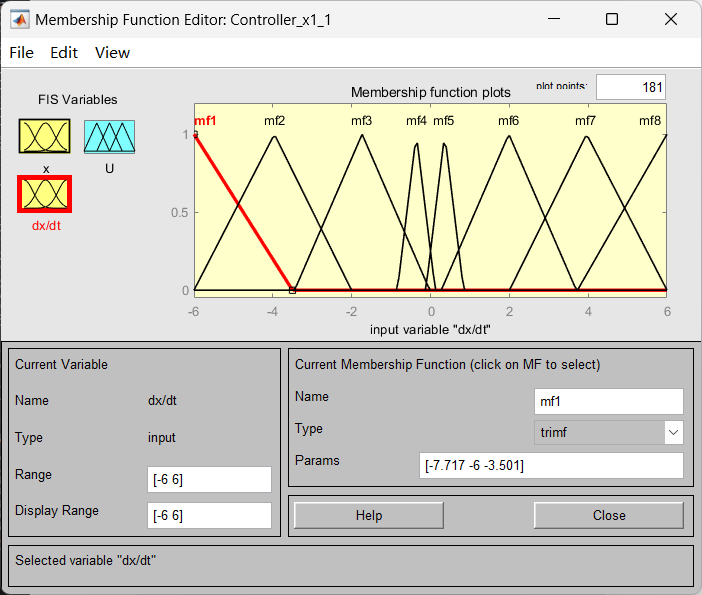
\includegraphics[width=0.32\textwidth]{figures/2024-12-13-22-15-28.png} 
         
    }%
        \subcaptionbox{U}[0.33\textwidth][c]{
        \centering
        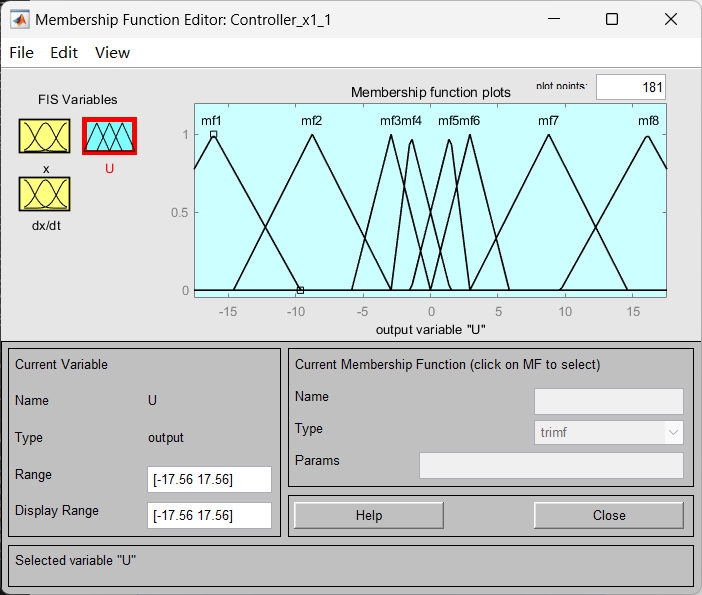
\includegraphics[width=0.32\textwidth]{figures/2024-12-13-22-15-42.png} 
         
    }%
    \caption{最终fis文件}
     
\end{figure}



\clearpage
\section{实验结果表现与分析}

\begin{figure}[htbp] \centering 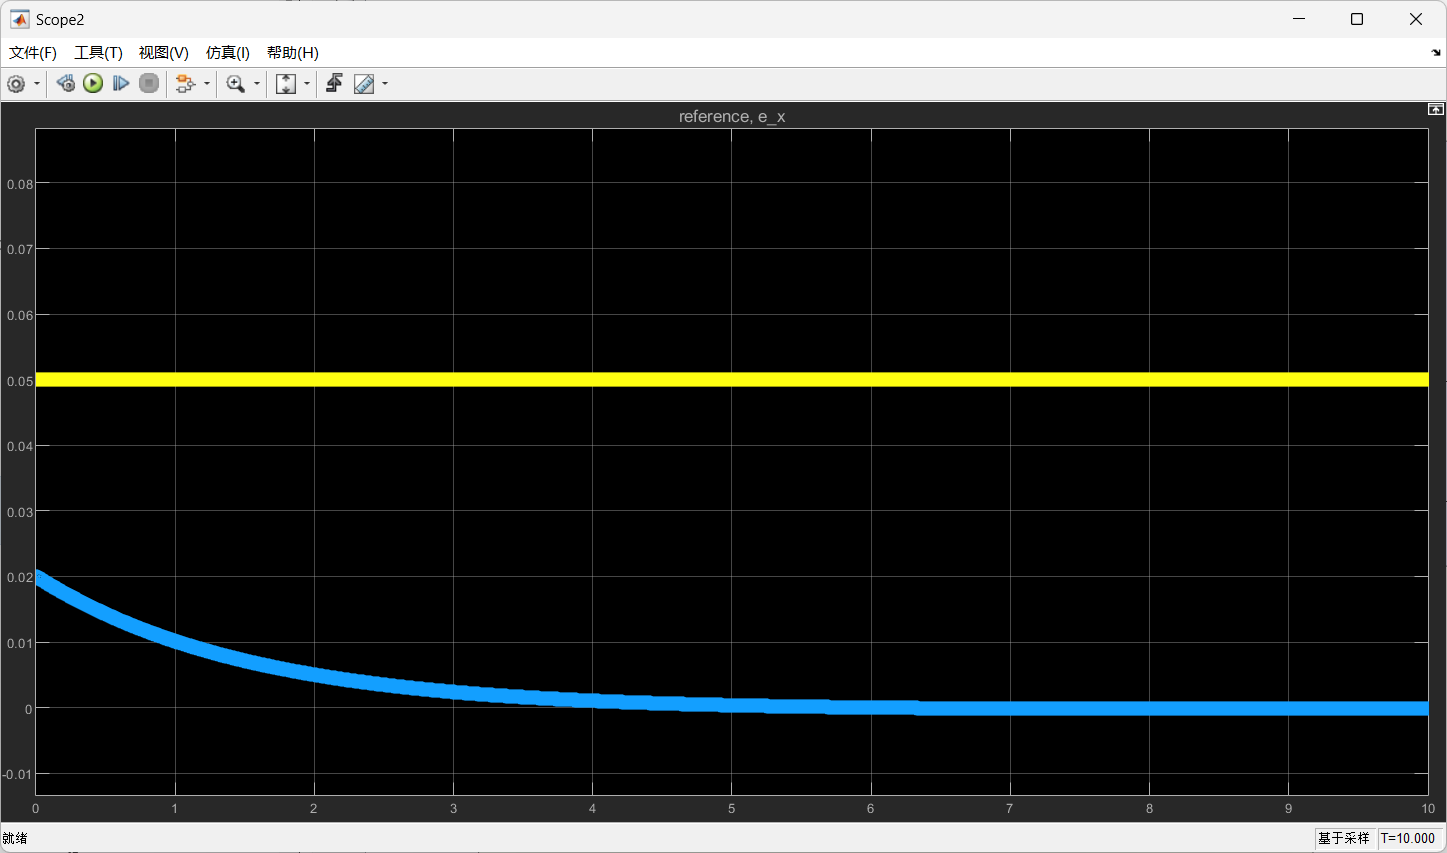
\includegraphics[width=0.5\textwidth]{figures/2024-12-13-22-21-18.png} \caption{reference add $e_x$}  \end{figure}

\begin{figure}[htbp] \centering 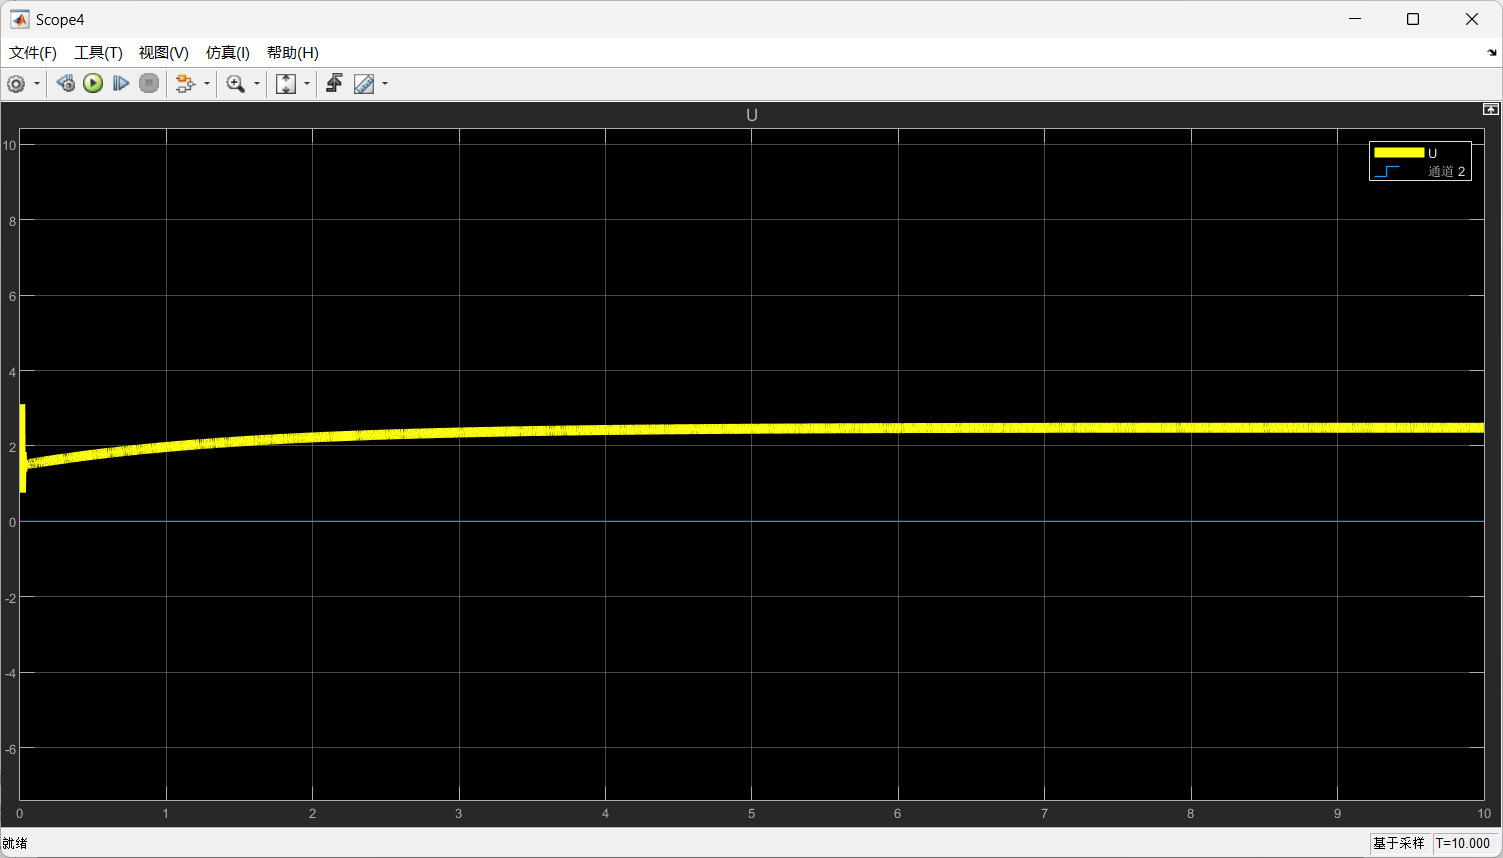
\includegraphics[width=0.5\textwidth]{figures/2024-12-13-22-22-07.png} \caption{$U$}  \end{figure}

\begin{figure}[htbp] \centering 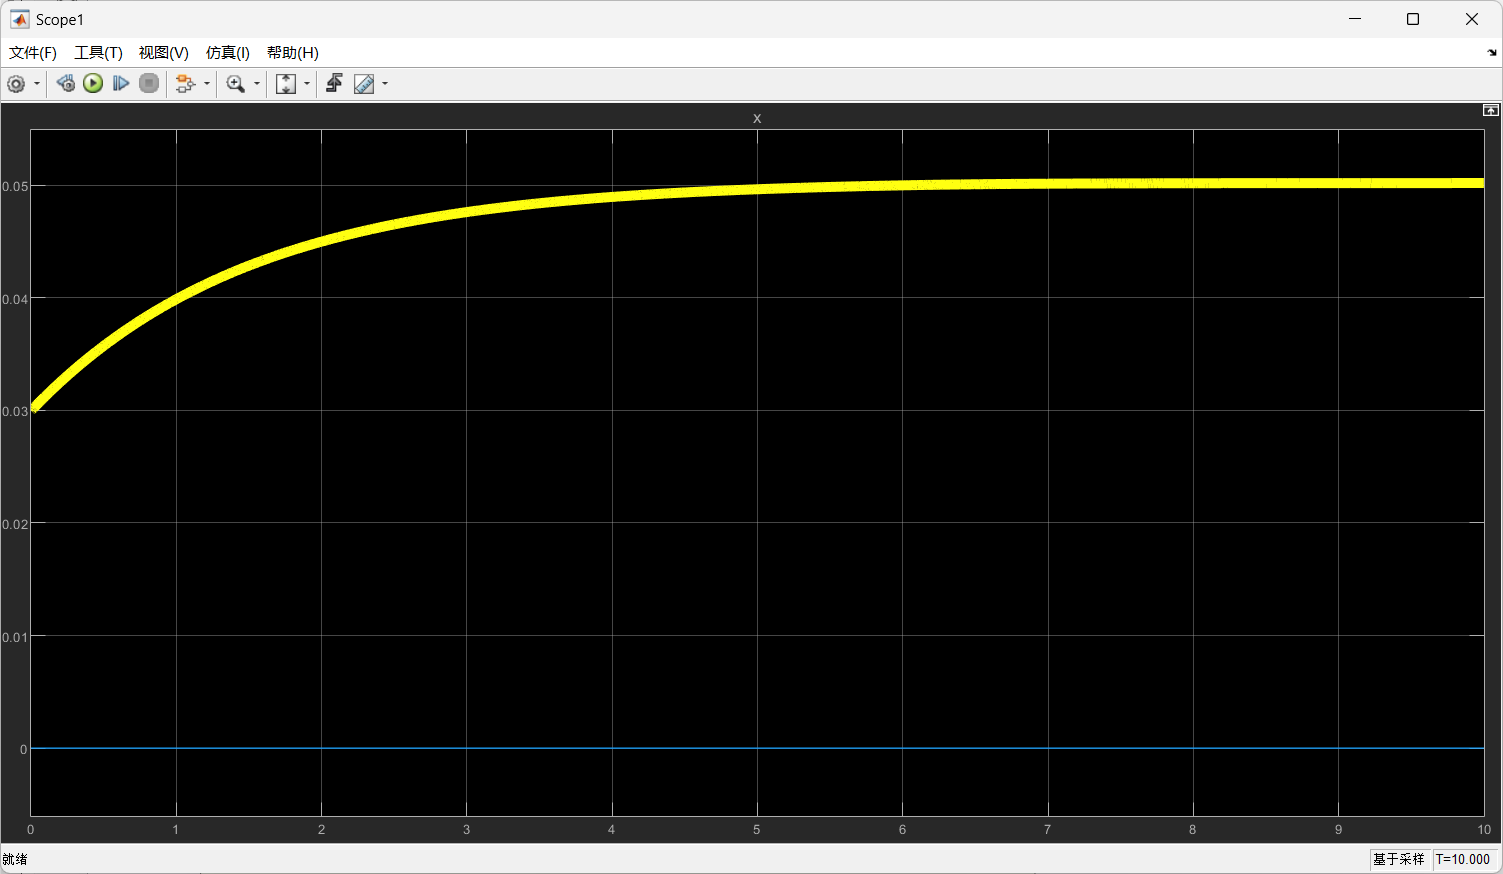
\includegraphics[width=0.5\textwidth]{figures/2024-12-13-22-22-41.png} \caption{$x$}  \end{figure}

从上面的仿真结果可以看出:

\begin{enumerate}
\item 系统响应性能良好。从图中可以看出,系统能够快速跟踪给定的参考输入信号,位置误差在短时间内就能收敛到参考位置附近。

\item 控制输出平稳。控制电压U的变化比较平滑,没有出现剧烈的震荡,这说明模糊控制器的规则库设计合理,控制作用适中。

\item 稳态精度高。在稳态时,位置x能够很好地跟随参考输入,稳态误差很小,满足控制要求。
\end{enumerate}

总的来说,所设计的模糊控制器实现了对磁悬浮系统的有效控制,系统表现出良好的动态性能和稳态性能。这验证了模糊控制在处理非线性系统时的优越性。


\subsection{$m = 0.1kg$}
更改到$m=0.1kg$后,经过调参以后,系统表现如下

\begin{figure}[htbp] \centering 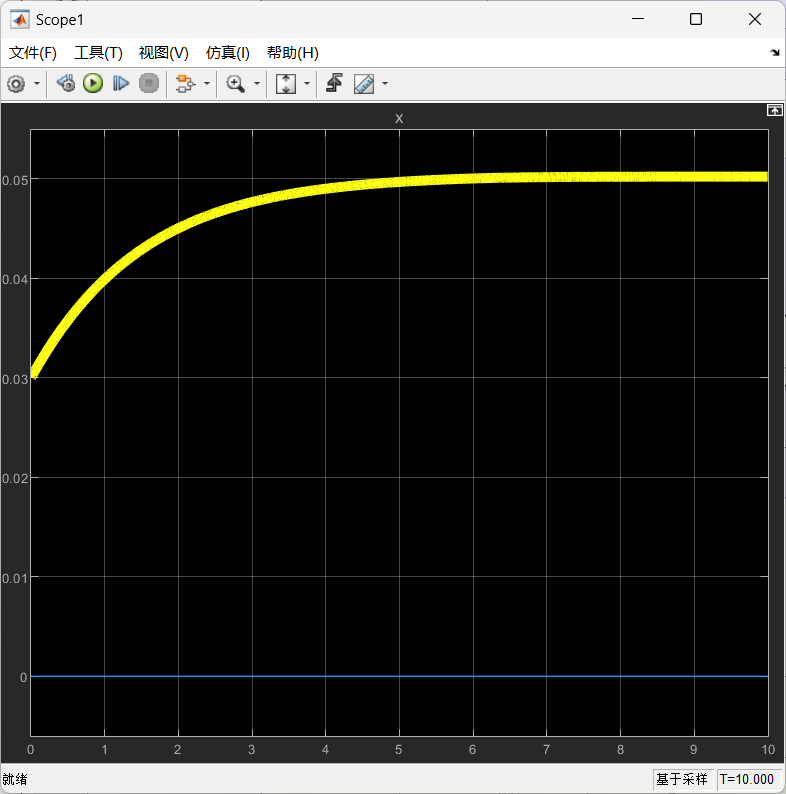
\includegraphics[width=0.7\textwidth]{figures/2024-12-13-23-46-34.png} \caption{m=0.1kg} \label{fig:m01} \end{figure}

可以看出系统可以稳定悬浮。

从图\ref{fig:m01}可以看出,当钢球质量增加到0.1kg时,系统仍然能够实现稳定悬浮,但是相比于m=0.05kg时:

\begin{enumerate}
\item 系统响应变慢。由于质量增大,系统的惯性也随之增大,导致系统响应速度变慢。

\item 控制电压增大。为了克服更大的重力,控制器需要输出更大的电压来产生足够的电磁力。
\end{enumerate}

为了适应钢球质量的变化,主要采取了以下调整措施:

\begin{enumerate}
\item 扩大控制电压的论域范围。原先控制电压的范围是[-20,20]V,为了适应更大的质量,将范围调整为[-27,27]V。这样可以提供更大的控制作用来克服增大的重力。

\item 保持位置误差和速度误差的论域几乎不变

\item 适当调整了模糊规则中的输出值大小,使控制作用更强。
\end{enumerate}

这些调整措施使得控制器能够较好地适应质量变化,保持系统的基本性能。但是从长远来看,更理想的解决方案是设计自适应模糊控制器,能够根据系统参数的变化自动调整控制参数。

\begin{figure}[htbp] \centering 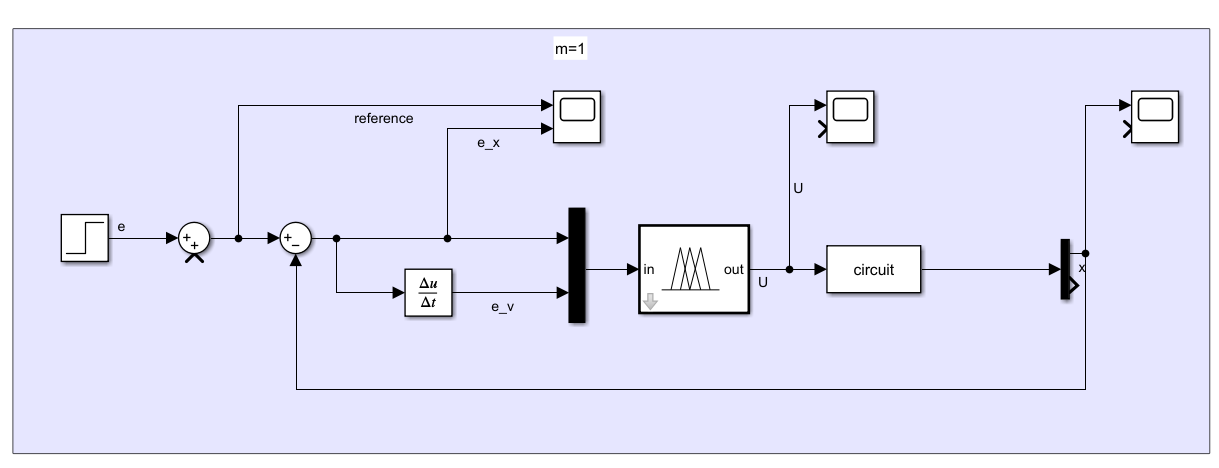
\includegraphics[width=0.7\textwidth]{figures/2024-12-13-23-51-42.png} \caption{m=0.1kg} \label{fig:m01} \end{figure}

\clearpage
\section{实验探究与可探索方向}

\subsection{动画仿真}

为了得到小球的真实运动轨迹,我还学习了simulink的3D Animation库,并把小球位置作为参数输入了VR 3D 中,最后效果如下图,还是比较有意思的。

\begin{figure}[htbp] \centering 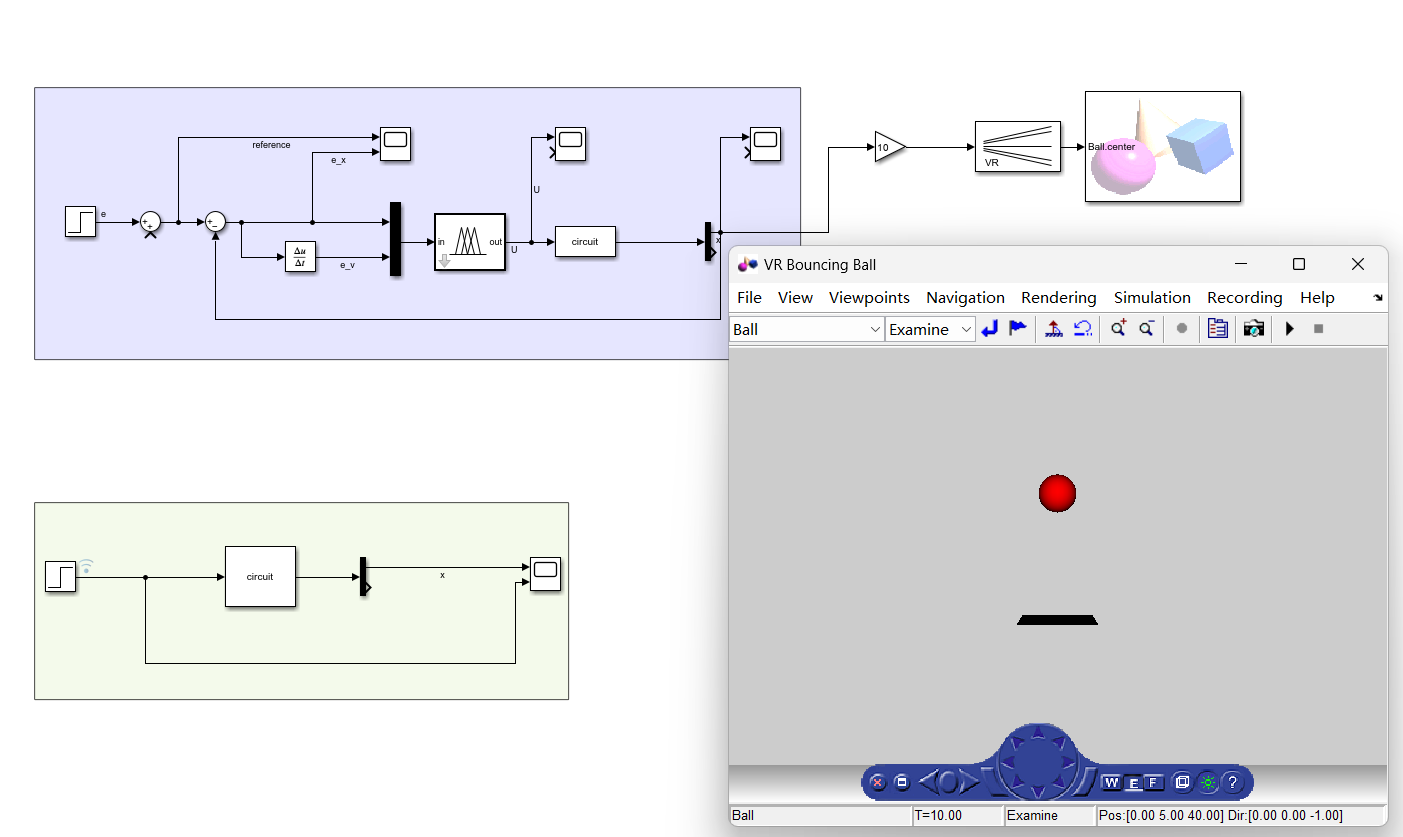
\includegraphics[width=0.9\textwidth]{figures/2024-12-13-22-27-25.png} \caption{3D Animation库}\end{figure}


\clearpage
\appendix
\section{附录1:源程序代码}

\dirtree{%
.1 .
.2 resources\DTcomment{资源文件夹}.
.2 circuit.m\DTcomment{磁悬浮系统仿真代码}.
.2 Controller\_x1\_1.fis\DTcomment{模糊控制器配置文件}.
.2 fis.m\DTcomment{模糊控制系统生成}.
.2 fuzz.slx\DTcomment{Simulink仿真模型}.
}

\begin{lstlisting}[language=Matlab,caption=fis.m]
clear;
close all;

% % 创建模糊推理系统,使用 newfis
% fuzzyController = mamfis( ...
%     'NumInputs',1,'NumInputMFs',2,...
%     'NumOutputs',1,'NumOutputMFS',2,...
%     'AddRule','none');
% 
% % 定义输入变量x(位置误差)及其隶属度函数,范围 [-0.04, 0.04]
% fuzzyController.Inputs(1).Name = 'x';
% fuzzyController.Inputs(1).Range = [-0.04 0.04];
% 
% fuzzyController = addMF(fuzzyController, 'input', 1, 'EN', 'gaussmf', [0.01 -0.04]); % EN: Extremely Negative
% fuzzyController = addMF(fuzzyController, 'input', 1, 'VN', 'gaussmf', [0.01 -0.03]); % VN: Very Negative
% fuzzyController = addMF(fuzzyController, 'input', 1, 'N', 'gaussmf', [0.01 -0.02]);  % N: Negative
% fuzzyController = addMF(fuzzyController, 'input', 1, 'NZ', 'gaussmf', [0.01 -0.01]); % Z: Zero
% fuzzyController = addMF(fuzzyController, 'input', 1, 'PZ', 'gaussmf', [0.01 0.01]);  % Z: Zero
% fuzzyController = addMF(fuzzyController, 'input', 1, 'P', 'gaussmf', [0.01 0.02]);   % P: Positive
% fuzzyController = addMF(fuzzyController, 'input', 1, 'VP', 'gaussmf', [0.01 0.03]);  % VP: Very Positive
% fuzzyController = addMF(fuzzyController, 'input', 1, 'EP', 'gaussmf', [0.01 0.04]);  % EP: Extremely Positive
% 
% % 可视化x的隶属度函数
% figure;
% subplot(311);
% plotmf(fuzzyController, 'input', 1);
% title('位置误差 (x) 的隶属度函数');
% 
% % 定义输入变量dx/dt(位置误差变化率)及其隶属度函数,范围 [-0.5, 0.5]
% fuzzyController.Inputs(2).Name = 'dx';
% fuzzyController.Inputs(2).Range = [-0.5 0.5];
% fuzzyController = addMF(fuzzyController, 'input', 2, 'EN', 'gaussmf', [0.1 -0.5]);  % EN: Extremely Negative
% fuzzyController = addMF(fuzzyController, 'input', 2, 'VN', 'gaussmf', [0.1 -0.4]);  % VN: Very Negative
% fuzzyController = addMF(fuzzyController, 'input', 2, 'N', 'gaussmf', [0.1 -0.3]);  % N: Negative
% fuzzyController = addMF(fuzzyController, 'input', 2, 'NZ', 'gaussmf', [0.1 -0.1]);     % Z: Zero
% fuzzyController = addMF(fuzzyController, 'input', 2, 'PZ', 'gaussmf', [0.1 0.1]);     % Z: Zero
% fuzzyController = addMF(fuzzyController, 'input', 2, 'P', 'gaussmf', [0.1 0.3]);   % P: Positive
% fuzzyController = addMF(fuzzyController, 'input', 2, 'VP', 'gaussmf', [0.1 0.4]);   % VP: Very Positive
% fuzzyController = addMF(fuzzyController, 'input', 2, 'EP', 'gaussmf', [0.1 0.5]);   % EP: Extremely Positive
% 
% % 可视化dx/dt的隶属度函数
% 
% subplot(312);
% plotmf(fuzzyController, 'input', 2);
% title('位置误差变化率 (dx/dt) 的隶属度函数');
% 
% % 定义输出变量U(控制电压)的隶属度函数,范围 [-10, 10]
% fuzzyController = addvar(fuzzyController, 'output', 'U', [-10 10]);
% fuzzyController = addMF(fuzzyController, 'output', 1, 'EL', 'trimf', [-10 -10 -7]);  % EL: Extremely Low
% fuzzyController = addMF(fuzzyController, 'output', 1, 'VL', 'trimf', [-10 -7 -4]);  % VL: Very Low
% fuzzyController = addMF(fuzzyController, 'output', 1, 'L', 'trimf', [-7 -4 -1]);   % L: Low
% fuzzyController = addMF(fuzzyController, 'output', 1, 'NZ', 'trimf', [-3 -1 1]);  % NZ:negetive ZERO
% fuzzyController = addMF(fuzzyController, 'output', 1, 'PZ', 'trimf', [-1 1 3]);  % M: positive ZERO
% fuzzyController = addMF(fuzzyController, 'output', 1, 'H', 'trimf', [1 4 7]);  % H: High
% fuzzyController = addMF(fuzzyController, 'output', 1, 'VH', 'trimf', [4 7 10]); % VH: Very High
% fuzzyController = addMF(fuzzyController, 'output', 1, 'EH', 'trimf', [7 10 10]); % EH: Extremely High
% 
% % 可视化U的隶属度函数
% 
% subplot(313);
% plotmf(fuzzyController, 'output', 1);
% title('控制电压 (U) 的隶属度函数');

fuzzyController = readfis('Controller4.fis');

table = [
    [1, 1, 1, 1, 6, 5, 5, 5],
    [1, 2, 2, 1, 7, 5, 5, 5],
    [2, 2, 2, 1, 2, 6 ,6, 6],
    [2, 3, 3, 2, 7, 6, 6, 6],
    [3, 3, 3, 2, 8, 7, 6, 7],
    [3, 3, 4, 2,8, 7, 7, 7],
    [3, 4, 4, 2, 8, 8, 7, 8],
    [4, 4, 4, 4, 8, 8, 8, 8]];
% 生成规则矩阵
rules = [];
for i = 1:8
    for j = 1:8
        disp(table(i,j));
        output = table(i,j);
        rules = [rules; i j  output 1 1]; % 1 1表示使用 'min' 合成和 'centroid' 解模糊
    end
end

% disp(rules)

% 添加规则到模糊系统
fuzzyController = addrule(fuzzyController, rules);
%showrule(fuzzyController,'Format','symbolic');
% 可视化规则
ruleview(fuzzyController);

%figure;
%plotfis(fuzzyController);

% 输出 surface
figure;
gensurf(fuzzyController,[1,2],1);
saveas(gcf, 'surf.jpg');



% 保存为.fis文件
writefis(fuzzyController, 'Controller41.fis');

testInputs = [0.01, -0.25];  % 例如,x=0.01, dx/dt=-0.25
output = evalfis(fuzzyController,testInputs);
disp(['控制电压U的输出:', num2str(output)]);
\end{lstlisting}


\begin{lstlisting}[language=Matlab,caption=物理系统实现]
    function [sys, x0, str, ts, simStateCompliance] = circuit(t, x, u, flag,m,g,K,R,L)
    % Critic S-Function
    % 输入:theta,目标值theta_target(无实际意义),
    % 输出:cost_function(基于最小theta的最大化)

    switch flag
        case 0
            [sys, x0, str, ts, simStateCompliance] = mdlInitializeSizes();
        case 1
            sys = mdlDerivatives(t, x, u,m,g,K,R,L);
        case 2
            sys = mdlUpdate(t, x, u);
        case 3
            sys = mdlOutputs(t, x, u);
        case 4
            sys = mdlGetTimeOfNextVarHit(t, x, u);
        case 9
            sys = mdlTerminate(t, x, u);
        otherwise
            DAStudio.error('Simulink:blocks:unhandledFlag', num2str(flag));
    end

    %% 子函数定义
    function [sys, x0, str, ts, simStateCompliance] = mdlInitializeSizes()
        % 初始化回调子函数
        
        sizes = simsizes;
        sizes.NumContStates = 3;   % 连续状态数
        sizes.NumDiscStates = 0;   % 离散状态数:[theta_min, cost_function]
        sizes.NumOutputs = 2;      % 输出个数
        sizes.NumInputs = 1;       % 输入个数
        sizes.DirFeedthrough = 0;  % 允许直馈通道
        sizes.NumSampleTimes = 1;  % 采样时间数
        sys = simsizes(sizes);     % 返回sizes数据结构
        x0 = [0.03 0 0];             % 初始状态:
        str = [];                  % 保留参数
        ts = [0 0];                % 采样时间
        simStateCompliance = 'UnknownSimState'; % 仿真状态合规性
    end

    function sys = mdlDerivatives(t, x, u,m,g,K,R,L)
        % 导数回调子函数(不使用,空实现)
        xx = x(1);
        dx = x(2);
        I = x(3);
        

        x_dot = dx;
        x_dot2 = (K * I^2 / xx^2 - m*g)/m;
        I_dot = (u - K*I/xx*dx - I*R)/L;
        
        %disp(u)
        %disp([x_dot;x_dot2;I_dot]);
        %disp(xx);
        sys = [x_dot;x_dot2;I_dot];
    end

    function sys = mdlUpdate(t, x, u)
        sys = [];
    end

    function sys = mdlOutputs(t, x, u)
        sys = [x(1);x(2)];
    end

    function sys = mdlGetTimeOfNextVarHit(t, x, u)
        % 计算下一个采样时间(定时采样)
        sampleTime = 1;  % 固定采样时间(1秒)
        sys = t + sampleTime;  % 下一次采样时间
    end

    function sys = mdlTerminate(t, x, u)
        % 仿真结束时的回调(输出成本函数)
        sys = [];
    end
end
\end{lstlisting}

\newpage
\section{附录2:版本更新记录}

\begin{table}[htbp]
    \centering
    \begin{tabular}{|l|p{12cm}|}
        \hline
        日期 & 更新内容 \\
        \hline
        2024.12.4 & 初始化项目;完成基本的模糊控制器设计;搭建Simulink仿真模型 \\
        \hline
        2024.12.8 & 优化模糊控制规则;调整隶属度函数参数;完善仿真模型 \\
        \hline
        2024.12.10 & 添加3D Animation动画效果;完成不同质量下的对比实验 \\
        \hline
        2024.12.13 & 完成论文撰写;添加实验数据分析;整理实验结果图表;完善文档格式 \\
        \hline
    \end{tabular}
    \caption{版本更新记录}
\end{table}

\nocite{*}
\bibliographystyle{unsrt}
\bibliography{ref}

\end{document}